\documentclass[]{article}
\usepackage{ctex}
\usepackage{graphicx}

%opening
\title{编译原理项目2}
\author{林伟业 20152100121}

\begin{document}

\maketitle

\section{编程语言}

Python

\section{开放工具}

sublime,Python,cmd

\section{实验内容}
比特大战

\section{程序文件}

main.py

\section{程序函数说明}

用list结构保存A和B的比特选择,然后两个list对应位置对比,按照表的得分算出A和B的总得分。

程序主函数main。类Bit\_war,定义对战方的属性和方法,方法是策略1到5。函数count\_score(num, a\_list, b\_list),统计A和B的总得分。函数A12(num),A用策略1和2与B用策略12345对战。函数A3(num),A用策略3与B用策略12345对战。函数A4(num),A用策略4与B用策略12345对战。函数A5(num),A用策略5与B用策略12345对战。函数A4(num),A用策略4与B用策略12345对战。函数B12345(num, a\_list),定义B的策略12345。

\section{程序运行截图}
\begin{figure}[h]
	\centering
	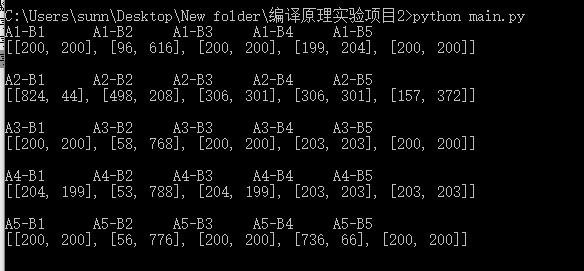
\includegraphics[width = 1\textwidth]{run.PNG}
	\caption{运行结果}
\end{figure}

\end{document}
